One of the most important aspects of any technology is how a human interacts with it.
Having an intuitive, simple, and functional interface can often be the difference between
a successful device and one which isn't. This importance on a interface is even more important
when trying to help someone with an impairment. Not only does the interface have to be all
the things mentioned above, but it also has to be robust for different environments. In the
case of assisting a person with visual impairment this means being able to handle cases
which people without visual impairment handle without even realizing they do. Such a scenario
would be when reaching for a product if you momentarily move your head in a different direction.

Our visual assistive system consists of several interacting components: 

\begin{itemize}
\item One of the devices that we use an off the shelf androdi powered smart glasses. 
The smart glasses have both a camera and a built in headset along with
networking capability. 
\item We use a specially designed prototype glove that has been
modified to have both a camera attached to it, as well set of
vibration motors. 
\item Smart Cart. A shopping cart that can be equiped with a moderate level of computer
and a variety of sensors that would be provided by the retail location.
\item High-performance server machine with both GPU and FPGA integration running
accelerating compute with custom algorithms and architectures.
\end{itemize}
\subsection{Interfaces}
For our assistive technology we employ two main modes of providing this feedback and guidance to the user. these modes are auditory feedback and tactile feedback. To provide this feedback to the users we use glove and glass listed above.
\subsubsection{Smart Glasses}
The off the shelf smart glasses provide the system with a camera in the viewpoint
of the persons head as well as network connectivity and speakers for audio feedback.
In the assistive system the glasses are mainly used to guide the person at the aisle level
to be infront of their intended/desired product. The commands such as "left, right, forward, back"
provide the direction. 
\subsubsection{Custom Glove}
The custom glove has both a camera and a series of vibration motors.
This camera that is on the glove allows the system to have the view
 point of where the person is reaching. This view point may be different from
that of the camera mounted on the headset and is critical to being able to provide
guidance all the way to physically picking up the intended product.
The vibration motors attached to the glove allow the system to provide
subtle feedback to the user the convey to them which when they would
have to move their hand to be able to grab the desired product. An
example of this would be buzzing the right motor to indicate a
rightward motion or the top motor to indicate the person needs to lift
their hand.

Figure~\ref{tab:whole_system_chris} shows how a person would wear and interface with the asssitive system. Such a system is ideal
to provide guidance and assistance in a retail type setting. <--- please change this line.

%Whole system picture
\begin{figure}[!htb]
\centering
\begin{tabular}{@{\hspace{1em}}l@{} @{\hspace{1em}}l@{}}
\vspace{-5pt}
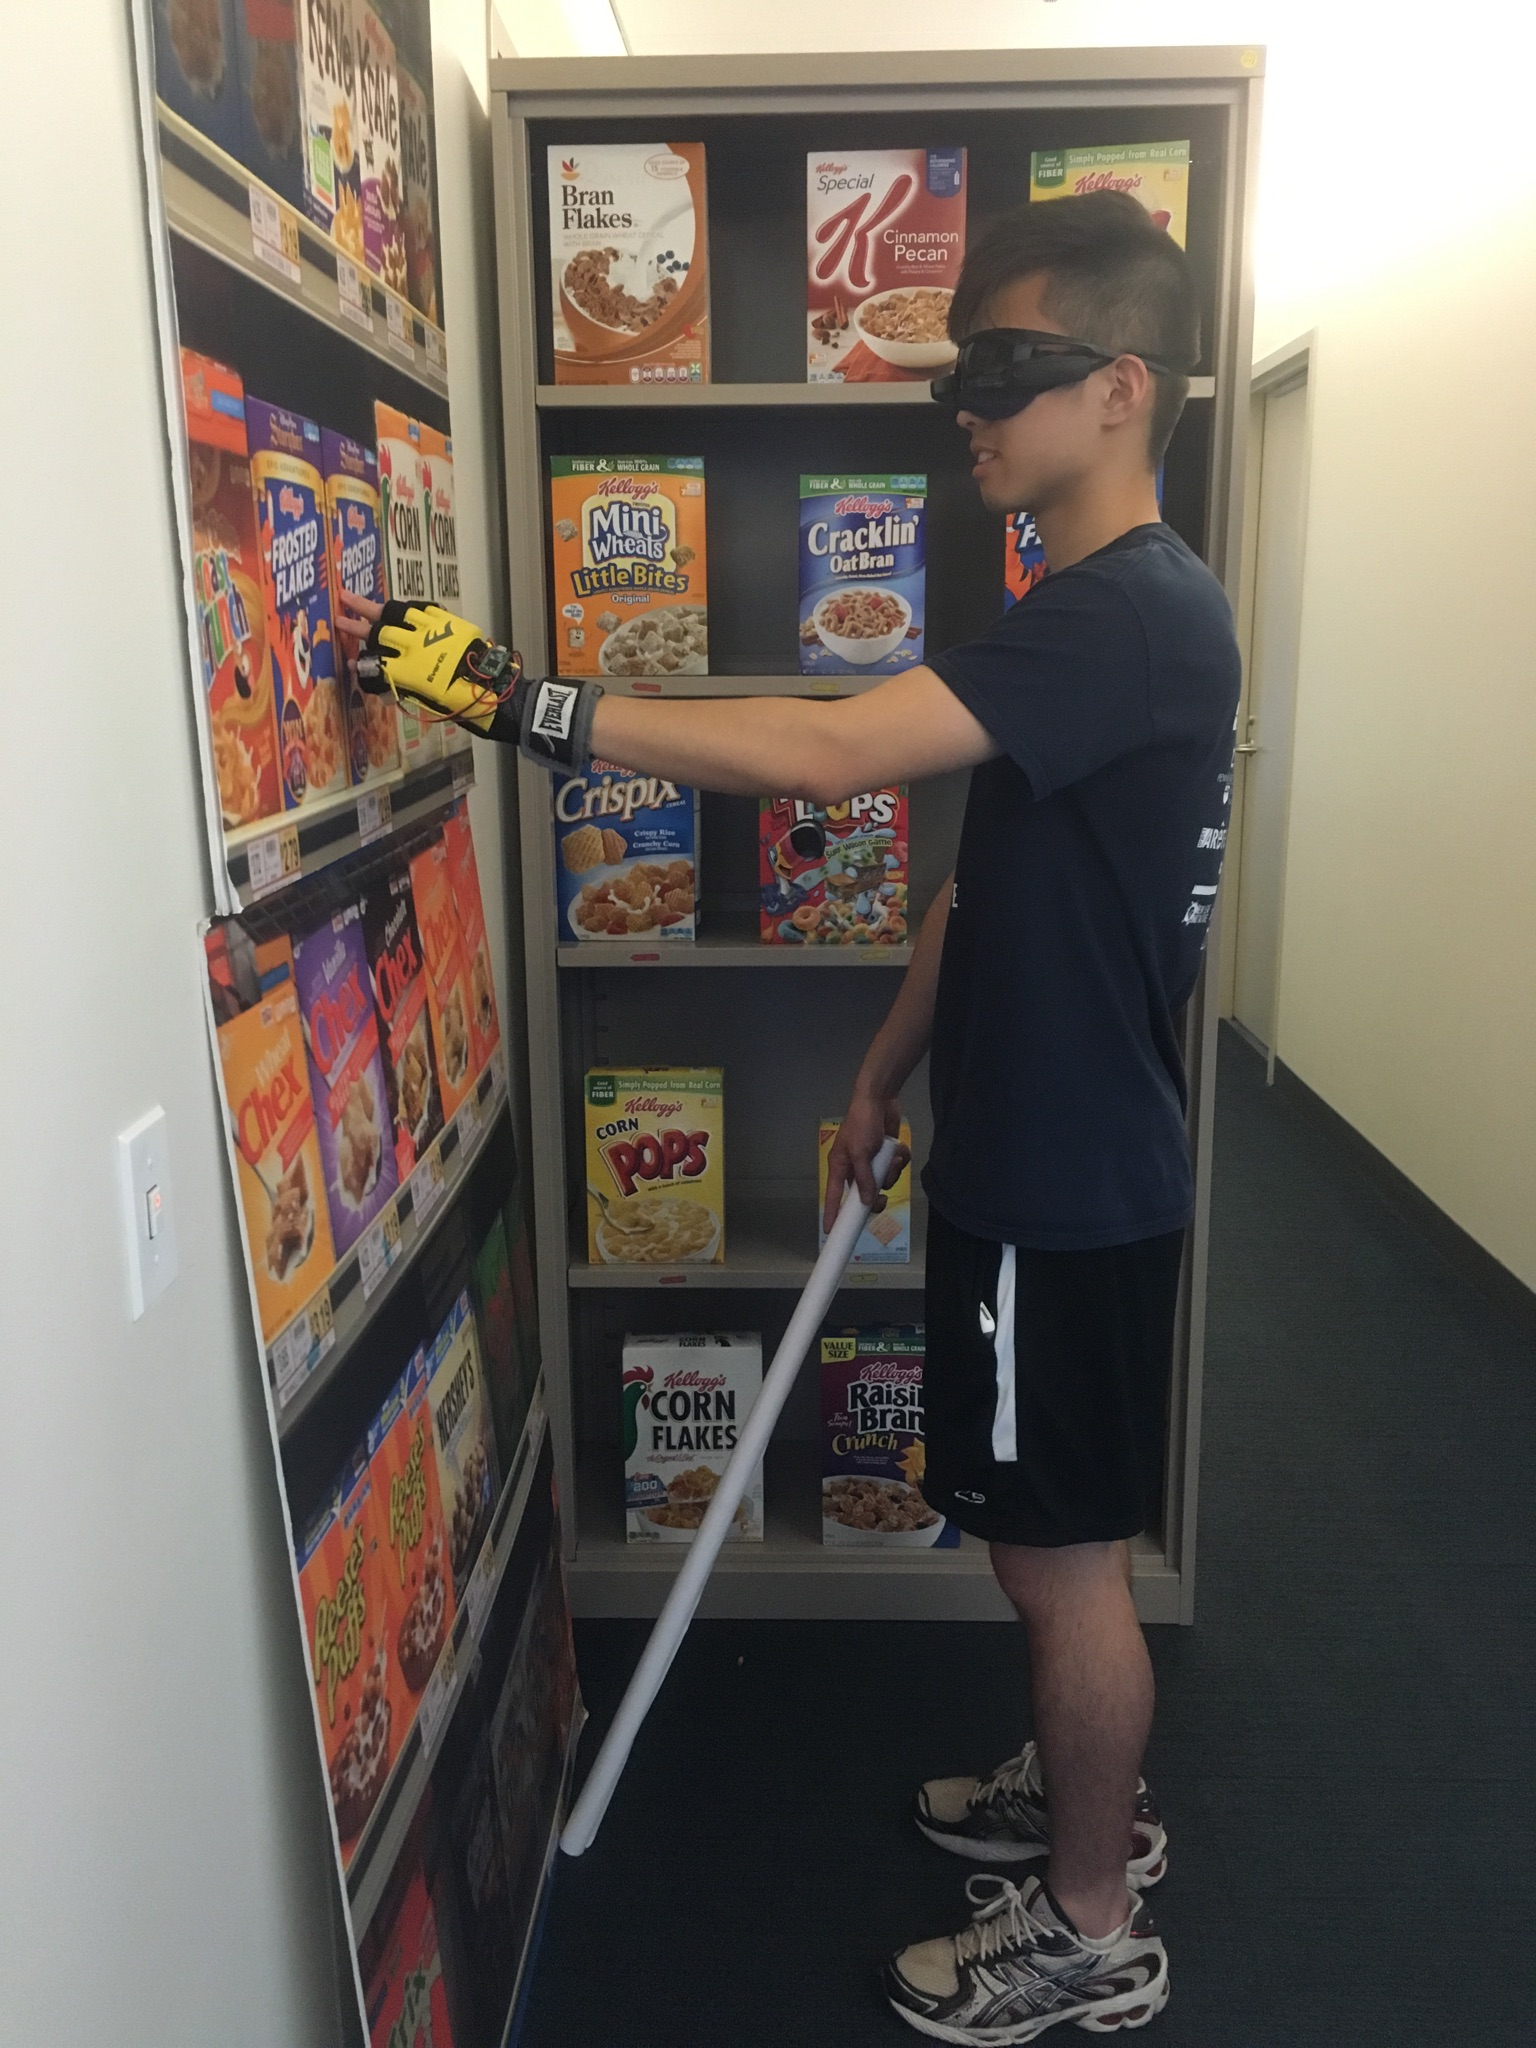
\includegraphics[width=0.9\linewidth,trim={0 0 0 0},clip]{chris_system_whole.jpg}\\[\abovecaptionskip]
\end{tabular}
\caption{ A person using an assistive system using multiple modes of feedback.}
\label{tab:whole_system_chris}
\end{figure}

\subsection{Using the System}
While certain aspects of system use differ across the particular tasks it supports, the modes and mechanisms employed during grocery shopping provide good coverage of typical operations, and we describe them in detail below.
In the our system these the auditory feedback combined with the haptic feedback from the glove
to provide the needed assistance to the shopper. 
 
\subsection{Challenges}
Creating a truly assistive system with a variety of interfaces presents a series 
of challenges, not all of which are intially obvious. These challenges include, guiding the person
through the store which includes, localization, obstiacle and person avoidance. Other challenges are
user centric. These include adapting the frequency of guidance commands to the speed at which the person is moving, 
reconciling different camera views to provide correct guidance, and having enough computational power to keep the system real-time. 
Through various methods these challenges can be solved. To solve the problem of guiding the person through the store, the smart cart could be equipped with various sensors. This could include cameras that not only have RGB information, but even depth and possibly thermal. Also the use of
localization technologies such as indoor gps, and bluetooth beacons around the store have the ability to track the user and provide the needed level of localization to the system.
Another challenge that arose came from having two camera views that aren't always in alignment with one another. An example of when is occurs is when shopping and you go to grab a product, you might look away while still reaching in towards your intended product. This poses a challenge to a system giving guidance based on the view from those cameras. One possible solution to this issue would be the addition of sensors to the glasses and the glove. The addition of an IMU and Magnomter to both of the edge compute give ability to correctly give guidance in these cases. An a example how this would work is if the headset camera view indicated the person needed to move right, but the glove camera was pointing straight. The system would be able tell the user to turn just their head to align the two views.
The biggest challenge that exists in a guidance system is being able to keep up with the real-time demands of the user. With an assistive system, meeting solving this is crucial. In order to do this effectively, the system as a whole must leverge every availble compute power including that available at both the edge devices, the local infastructure in addition to a powerful cloud compute platform. As stated earlier, for our cloud compute device use a high-performance server that is enabled/enhanched with both FPGAs and GPUs. By leverageing custom architecures and exploiting parrallel algorithms we are able to process 1080p at ~50fps. While this may seem like it meets the real-time constratint it doesn't. Since a server needs to be able handle multiple connections at once, just the acclerated back end would handle 50 streams at 1fps. To make up this gap in performace, tricks need to be played at the local and edge compute devices to make this difference imperceivable. Some of the compute that 





User movement speed:
With any system that provides user feedback, being able to keep up with the speed at which the user moves. In a system that is meant to provide assistance and guidance the fluidity of the interface is crucial. The slightest delay in this type of system could lead to a variety of situations such as the user walking into something, missing the intended product, or picking the wrong product. In a task that requires image processing this problem is even more difficult due to the computation requriement of the backend.



